Der folgende Abschnitt behandelt ein spezielles Verfahren der evolutionären Optimierung. Das CMA-ES-Verfahren. Es stellt den "State of the Art"- der Evolutionären Berechnungsverfahren dar. Für spezialisierte Probleme gibt es bessere Lösungen, als allgemeiner Solver für unregistrierte, kontinuierliche Probleme ist dieses Verfahren mehr als tauglich. Es wurde um die Jahrtausendwende entwickelt und veröffentlicht. Typische Einsatzgebiete der CMA-ES sind unregistrierte Optimierungsprobleme mit einem Suchraum zwischen drei und einhundert Dimensionen. Der Algorithmus kann eingesetzt werden wenn auf Ableitung angewiesene Verfahren (z.B. Newtonverfahren) aufgrund zerklüftete Suchräume, Rauschen, viele lokale Optima oder Ausreißern zu Fehlern neigen. Die Methode ist geeignet für nicht separierbare, schlecht konditionierte Probleme. Das Verfahren benötigt keine Gradienten, oder erfordert ihre Existenz. Dadurch kann der Algorithmus auch auf nicht stetige Probleme angewandt werden. Es existieren verschiedene Abwandlungen des Algorithmus, die für spezielle Fragestellungen geeigneter sind, und sogar eine Lösung zur Multiobjekt-Optimierung (MO-CMA-ES) wurde beschrieben~\cite{HansenMOO:1}. Das Verfahren wird aktuell stets weiterentwickelt~\cite{hansen2004ecm,hansen2009bbi}. Das Verfahren wurde in vielen Fragestellungen angewendet, eine unvollständige, etwas veraltete Übersicht ist unter \cite{CMAESOverview} zu finden.
%
%------------------------------------------------------------------
\begin{figure} [ht!]
\centering
         \caption[Konzept direkter Optimierung mittels CMA-ES]{Die Abbildung zeigt sechs Lösungsschritte des CMA-ES-Verfahrens. Eingangs wird eine Population mit einer Gauß-Verteilung generiert. Diese bewegt sich in jeder Generation näher an das globale Optimum heran. Die gestrichelte Linie zeigt dabei eine Isolinie der Wahrscheinlichkeitsdichte. Wir befinden uns auf einem 2D-Problem, somit wird das vorankommen der Population über zwei $\sigma$'s gesteuert. Dadurch kommt die Ellipse zu Stande. Die Linie bedeutet nicht, dass nur in diesem Bereich Nachkommen erzeugt werden, siehe z.B. Generation 4. Je nach Beschaffenheit des Problems und nach Nähe zum Optimum werden die steuernden $\sigma$'s kleiner. \cite{Wiki:Images:1}}
         \label{fig:conecpt_cma.es}
         \vspace{0.5cm}
         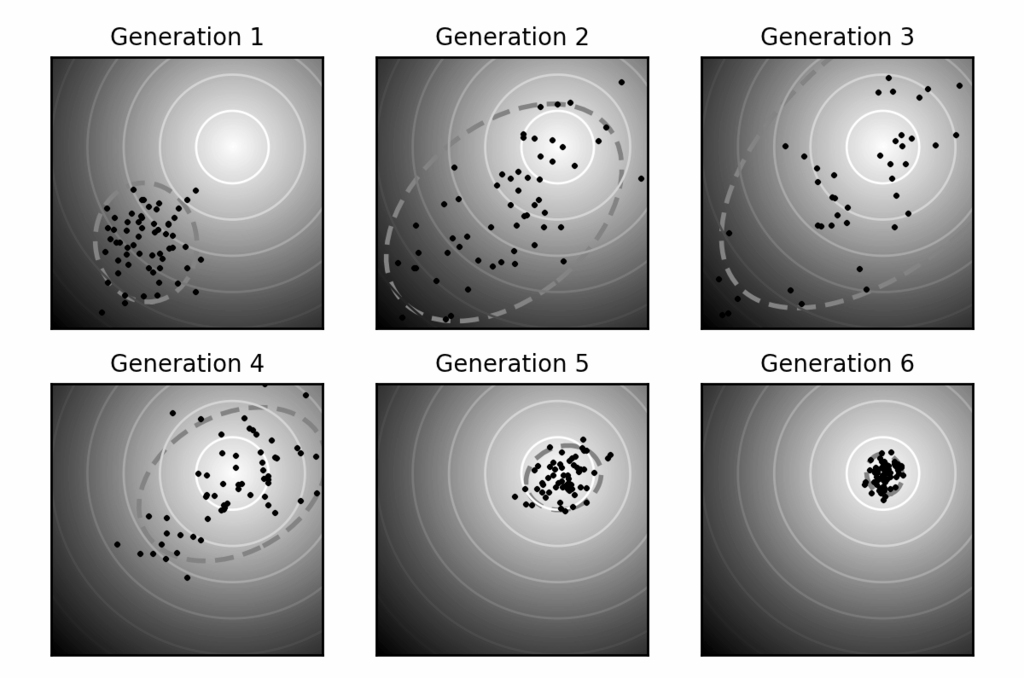
\includegraphics[width=\textwidth]{img/CMA-ES_algorithm.png}
%      
\end{figure}

%
Durch die Anpassung der Kovarianz-Matrix wird eine enge Abschätzung der Konturlinien der Objektfunktion $f$.\\

%
Der Algorithmus steht in verschiedene Implementationen, Programmiersprachen und Umgebungen zur Verfügung \cite{HansenCode}. Teilweise sind die Implementationen proprietär (z.B. Matlab), teilweise quelloffen. Die in dieser Arbeit zur Anwendung kommende Umsetzung ist die Shark-Library. Diese Bibiliothek ist eine in \cpp  geschriebene, quelloffene Software, die am Institut für Neuroinformatik der Ruhr Universität Bochum entwickelt wird. Detailliert wird Shark im Rahmen des Hauptteils in Abschnitt~\ref{sec:Shark} vorgestellt.
